% Trabajo final — Deep Learning
% Compilar en Overleaf con pdfLaTeX. Sin dependencias fuera de los paquetes
% estándar de TeX Live, y con la bibliografía embebida para que no haga falta
% ejecutar BibTeX por separado.
%
% Las figuras se buscan en ./figures/ y en ../figures/, así que funciona tanto
% subiendo el proyecto entero a Overleaf como copiando solo esta carpeta.

\documentclass[twocolumn,10pt,a4paper]{article}

\usepackage[utf8]{inputenc}
\usepackage[T1]{fontenc}
\usepackage[spanish,es-tabla,es-nodecimaldot]{babel}

\usepackage{amsmath,amssymb}
\usepackage{graphicx}
\usepackage{booktabs}
\usepackage{caption}
\usepackage[margin=2.2cm]{geometry}
\usepackage{xcolor}
\usepackage[colorlinks=true,allcolors=blue!60!black]{hyperref}

\graphicspath{{figures/}{../figures/}}

\captionsetup{font=small,labelfont=bf}
\setlength{\parskip}{0pt}

% Notación recurrente.
\newcommand{\R}{\mathbb{R}}
\newcommand{\norm}[1]{\left\lVert #1 \right\rVert}
\newcommand{\abs}[1]{\left\lvert #1 \right\rvert}

\title{\vspace{-1.2em}\textbf{Transformadas de scattering: invarianza sin
aprendizaje}\\[0.2em]
\large Una réplica del experimento de pocos datos de Bruna y Mallat}

\author{Andrés Felipe Barreto Farfan\\[0.2em]
\small Trabajo final — Matemáticas del aprendizaje de máquinas}

\date{\small{29 de julio de 2026}}

\begin{document}
\maketitle

\begin{abstract}
\noindent
La transformada de scattering de Bruna y Mallat construye representaciones
invariantes a traslaciones y estables frente a deformaciones mediante una
cascada de convoluciones wavelet, módulo y promediado, sin aprender
ningún parámetro. Esto sugiere una ventaja si tenemos pocos datos, donde
una red convolucional tiene más capacidad que evidencia. Replicamos su
experimento sobre MNIST con código propio y comparamos frente a una red
convolucional entrenada con prácticas actuales, bajo un protocolo idéntico para
todos los modelos y con cinco semillas por configuración. Se reprodujeron sus
cifras con una diferencia media menor a 0,3 puntos, pero la ventaja del scattering resulta más estrecha de lo publicado por Bruna y Mallat, es concluyente entre $1000$ y $2000$ muestras y
desaparece en ambos extremos, incluido $n=300$, donde además su varianza
cuadruplica la de la red.
\end{abstract}

\section{Introducción}

Las redes convolucionales funcionan muy bien, y no está del todo claro por qué.
Una explicación atribuye su éxito a los pesos que aprenden. Otra lo atribuye a la
arquitectura misma, la forma de encadenar convoluciones, no linealidades y
submuestreo ya encaja con la estructura de las imágenes naturales, casi con
independencia de qué filtros se usen. Saber cuál de las dos pesa más no es fácil,
porque en una red corriente ambas van de la mano.

La transformada de scattering \cite{bruna2011,bruna2013} permite poner a prueba
      esa segunda hipótesis, porque es exactamente una red convolucional cuyos filtros
están fijados por construcción y en la que no se aprende nada. Si una red
así compite con una entrenada, entonces buena parte del mérito corresponde a la
arquitectura.

Este trabajo replica el experimento central de \cite{bruna2013} sobre MNIST y lo
contrasta con una red convolucional entrenada end-to-end. Lo que nos interesa es cómo se comporta cada modelo
cuando los datos escasean, que es donde la ausencia de parámetros debería
notarse. Todo el código y los resultados intermedios están disponibles.%
\footnote{\url{https://github.com/afbarretof/Transformada-scattering.git}}

\section{La transformada de scattering}

\subsection{Construcción}

Recogemos aquí la construcción de \cite{bruna2013}, cuyo fundamento teórico
desarrolla \cite{mallat2012}, la notación es la de estos trabajos. La meta es
convertir una imagen en una lista de números (un descriptor) que apenas
cambie cuando la imagen se desplaza un poco o se deforma ligeramente, pero que
siga distinguiendo un dígito de otro. La construcción alcanza esas dos cosas a la
vez encadenando tres operaciones sencillas, convolución con wavelets, módulo y
promediado.

Una \emph{wavelet} es un filtro localizado que oscila unas pocas veces y luego
decae, con media nula. Puede pensarse como un pequeño detector de un trazo de
cierto grosor y cierta inclinación. Su media nula la hace ciega a un fondo
constante y sensible solo a las variaciones (bordes, trazos, texturas), al
convolucionarla con una imagen, la respuesta $x * \psi$ mide en cada punto cuánta
oscilación de esa forma hay a su alrededor. La wavelet está concentrada en el espacio, de
modo que su respuesta es local.

 A partir de una única wavelet madre compleja $\psi$ se genera un banco de filtros
dilatándola y rotándola,
\begin{equation}
  \psi_{j,\theta}(u) = 2^{-2j}\,\psi\!\left(2^{-j} r_{-\theta}\, u\right),
\end{equation}
que depende de dos parámetros. La escala $2^j$ fija el tamaño de los
detalles a los que responde el filtro, a mayor $j$, estructuras más grandes. La orientación $\theta$, una de $L$ direcciones que reparten el
plano mediante la rotación $r_\theta$, fija a lo largo de qué eje oscila.
Escribimos $\lambda = (j,\theta)$ para un índice del banco de wavelets, cuyos elementos
aparecen en la figura~\ref{fig:filtros}.

La respuesta $x * \psi_\lambda$ oscila y depende de la posición, para extraer de
ella una medida estable se le aplica el módulo $\abs{\cdot}$, que conserva
la amplitud de la oscilación y descarta su fase. El operador elemental de la
cascada combina ambas operaciones,
\begin{equation}
  U[\lambda]x = \abs{x * \psi_\lambda},
\end{equation}
y se itera a lo largo de un camino $p = (\lambda_1,\dots,\lambda_m)$,
aplicando en cada paso una wavelet distinta seguida del módulo,
\begin{equation}
  U[p]x = U[\lambda_m]\cdots U[\lambda_1]x .
\end{equation}
Por último, cada camino se promedia con un filtro paso bajo $\phi_J$ (un
filtro sin oscilación que difumina a la escala $2^J$, borrando la posición exacta
y ganando así invarianza a traslaciones), lo que produce los coeficientes
de scattering:
\begin{equation}
  S_J[p]x = U[p]x * \phi_J .
  \label{eq:scattering}
\end{equation}

El \emph{orden} $m$ de un coeficiente es la longitud de su camino. El orden $0$
es el simple promedio $x*\phi_J$, es decir una versión difuminada de la imagen.
Un coeficiente de orden $1$ resume cuánta oscilación de una escala y orientación
dadas hay en cada región, cuántos bordes finos verticales, cuántos trazos
gruesos diagonales, y así sucesivamente. Uno de orden $2$
describe cómo se organizan esos bordes a una escala mayor (por ejemplo, si los
trazos finos que detectó el primer filtro forman a su vez un patrón regular),
información que el promediado del orden $1$ ya había borrado.

\subsection{Módulo}

El promediado con $\phi_J$ da la invarianza a traslaciones que buscamos, pero al
difuminar borra el detalle fino. Si nos quedáramos solo con él, perderíamos casi
todo lo que distingue un dígito de otro. La convolución con la wavelet sí
conserva ese detalle, pero tiene el defecto opuesto: se desplaza junto con la
imagen, así que no es invariante. El módulo es lo que concilia ambas cosas. Como
$\psi$ es compleja, con parte real e imaginaria desfasadas un cuarto de ciclo, su
módulo $\abs{x * \psi_\lambda}$ es una
envolvente, la curva suave que sigue la amplitud de la oscilación sin sus
subidas y bajadas rápidas. Al ser una señal lenta, sobrevive al promediado donde
la oscilación original no lo haría. Dicho de otro modo, el módulo lleva la
información de detalle fino hasta un rango donde $\phi_J$ ya no la borra, y por
eso la cascada recupera lo que un solo promediado habría perdido.

Los coeficientes de
orden $1$ describen la energía local por escala y orientación. Los
de orden $2$ capturan cómo interactúan dos escalas distintas, información que
ningún promediado de orden $1$ puede representar porque precisamente la promedia.

\begin{figure}[t]
  \centering
  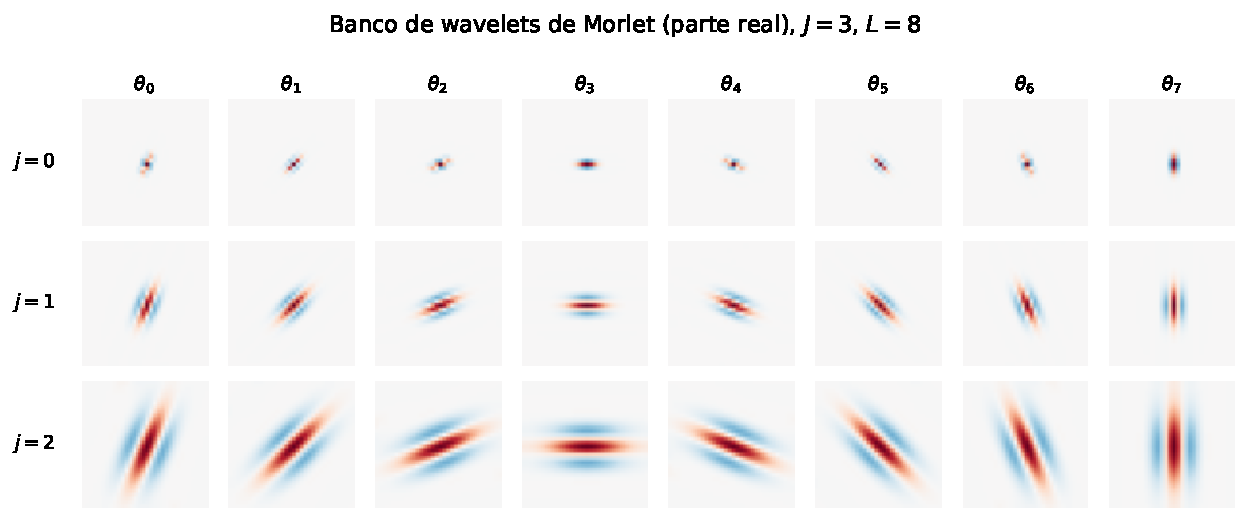
\includegraphics[width=\columnwidth]{fig01_filtros_espacial_real}
  \caption{Banco de wavelets de Morlet (parte real) para $J=3$ y $L=8$. Cada
  fila es una escala y cada columna una orientación. Los filtros no se aprenden:
  se obtienen dilatando y rotando una única wavelet madre.}
  \label{fig:filtros}
\end{figure}

\subsection{Invarianza y estabilidad}

El promediado con $\phi_J$ hace que el descriptor apenas cambie cuando la imagen
se desplaza, es casi invariante a traslaciones. Pero para clasificar dígitos
importa más otra propiedad, la estabilidad frente a deformaciones. Una
deformación no mueve el dígito entero, lo deforma localmente (un trazo que se
curva, un lazo que se ensancha). Mallat demuestra que, si la deformación es
suave, el descriptor cambia poco y en proporción a lo suave que sea
\cite{mallat2012}. Eso es justo lo que hace falta para clasificar, dos versiones
deformadas del mismo dígito quedan cerca en la representación. El módulo de la
transformada de Fourier, en cambio, falla aquí, porque una deformación pequeña
desplaza sus frecuencias altas y aleja las dos versiones.

\section{Metodología}

\subsection{Configuración}

Usamos MNIST \cite{lecun1998} con las imágenes centradas en un lienzo de
$32\times32$, y una
transformada de scattering con $J=3$ (es decir $2^J = 8$, el valor que
\cite{bruna2013} selecciona por validación cruzada) y $L=8$ orientaciones,
calculada con Kymatio \cite{kymatio}. El descriptor resultante tiene $217$
caminos sobre una rejilla espacial de $4\times4$, esto es $3472$ dimensiones
para el orden~2 y $400$ para el orden~1.

Comparamos cuatro modelos, una SVM con kernel gaussiano sobre los píxeles
crudos, una SVM sobre los coeficientes de scattering, el clasificador generativo
de espacios afines (PCA) de \cite{bruna2013} y una red convolucional entrenada
end-to-end.

El clasificador generativo de espacios afines (PCA) modela cada clase por
separado, toma los ejemplos de un dígito, calcula su centro (el \emph{centroide})
y las $d$ direcciones a lo largo de las cuales esos ejemplos más varían (sus
componentes principales, obtenidas por un PCA de la clase). El centro y esas direcciones definen un plano
afín $A_{d,k}$, un modelo compacto de la forma típica de la clase $k$ y de sus
variaciones. Para clasificar un descriptor $S x$ se mide su distancia a cada
plano (cuánto de $S x$ queda sin explicar tras proyectarlo sobre él,
$\norm{S x - P_{A_{d,k}}(S x)}$) y se le asigna la clase cuyo plano lo explica
mejor. Se llama generativo porque cada clase se ajusta por su cuenta, sin
trazar fronteras con las demás, al contrario que la SVM.

Los coeficientes de distintos caminos tienen magnitudes muy dispares, los de
orden bajo toman valores mucho mayores que los de orden~2. Como los dos
clasificadores comparan descriptores midiendo distancias, sin corregir esto un
coeficiente grande pesaría más que uno pequeño por su sola magnitud, aunque el
pequeño fuese más informativo. Por eso normalizamos los coeficientes antes de
clasificar y, siguiendo a \cite{bruna2013}, de forma distinta según el
clasificador. Para la SVM se reescala cada coeficiente al rango $[-1,1]$. Para el
clasificador afín se divide cada camino $p$ por el mayor valor que alcanza su
norma en el conjunto de entrenamiento, $\max_i \norm{S[p]X_i}$, con lo que su
ejemplo más intenso queda ajustado a $1$.

Ahora definamos las reglas para todos los modelos.

Primero, para cada tamaño $n$ se extrae una
submuestra estratificada y los cuatro modelos reciben exactamente los mismos
índices.

Segundo, validación cruzada de
tres pliegues dentro de esas $n$ muestras, seguida de un reajuste con las $n$
completas. Esto incluye a la red, cuyo número de épocas se elige promediando las
curvas de validación de los tres pliegues. Un solo conjunto de validación no
servía con pocos datos, con $n=300$ tendría apenas $60$ imágenes, y entonces la
época elegida dependía de si el modelo acertaba una o dos imágenes más, es decir,
del azar.

Tercero, todos los números se
promedian sobre cinco semillas.

\section{Resultados}

% Generado por scripts/consolidar.py — no editar a mano.
\begin{table*}[t]
  \centering
  \small
  \caption{Error de clasificación (\%) en MNIST según el tamaño del
  conjunto de entrenamiento. Media $\pm$ desviación típica sobre cinco
  semillas. Las dos últimas filas reproducen los valores publicados por
  Bruna y Mallat para referencia.}
  \label{tab:resultados}
  \begin{tabular}{lrrrrr}
    \toprule
    Modelo & $n=300$ & $n=1000$ & $n=2000$ & $n=5000$ & $n=10000$ \\
    \midrule
    píxeles + SVM & 13.56 $\pm$ 1.06 & 7.94 $\pm$ 0.26 & 5.77 $\pm$ 0.33 & 3.82 $\pm$ 0.13 & 2.89 $\pm$ 0.06 \\
    scattering orden 1 + PCA & 5.33 $\pm$ 0.20 & 2.85 $\pm$ 0.28 & 2.21 $\pm$ 0.08 & 1.91 $\pm$ 0.11 & 1.82 $\pm$ 0.05 \\
    scattering orden 1 + SVM & 7.26 $\pm$ 0.59 & 3.56 $\pm$ 0.37 & 2.49 $\pm$ 0.19 & 1.69 $\pm$ 0.16 & 1.26 $\pm$ 0.07 \\
    scattering orden 2 + PCA & 4.21 $\pm$ 0.61 & 1.46 $\pm$ 0.13 & 1.18 $\pm$ 0.04 & 0.99 $\pm$ 0.06 & 0.82 $\pm$ 0.02 \\
    scattering orden 2 + SVM & 5.33 $\pm$ 0.58 & 2.59 $\pm$ 0.25 & 1.91 $\pm$ 0.15 & 1.23 $\pm$ 0.11 & 0.97 $\pm$ 0.03 \\
    CNN entrenada & 4.17 $\pm$ 0.14 & 2.28 $\pm$ 0.18 & 1.70 $\pm$ 0.12 & 1.08 $\pm$ 0.10 & 0.77 $\pm$ 0.06 \\
    \midrule
    \emph{Bruna y Mallat, scattering orden 2 + PCA} & 4.70 & 2.30 & 1.30 & 1.03 & 0.88 \\
    \emph{Bruna y Mallat, ConvNet} & 7.18 & 3.21 & 2.53 & 1.52 & 0.85 \\
    \bottomrule
  \end{tabular}
\end{table*}


\begin{figure}[t]
  \centering
  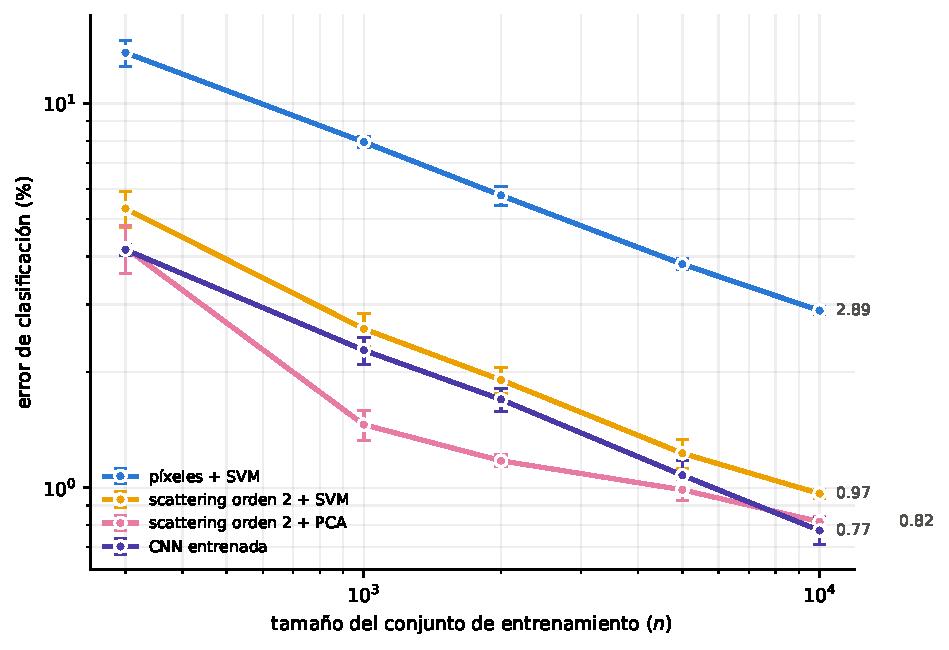
\includegraphics[width=\columnwidth]{fig08_curva_datos}
  \caption{Error de clasificación frente al tamaño del conjunto de
  entrenamiento. Las barras cubren una desviación típica sobre cinco semillas.
  Ambos ejes en escala logarítmica.}
  \label{fig:curva}
\end{figure}

\subsection{La réplica reproduce el original}

El cuadro~\ref{tab:resultados} muestra que nuestras cifras quedan próximas a las
publicadas. Para el scattering de orden~2 con clasificador afín obtenemos
$4{,}21\%$ frente al $4{,}70\%$ original con $n=300$, y $0{,}99\%$ frente a
$1{,}03\%$ con $n=5000$. La coincidencia es razonable teniendo en cuenta que
Kymatio no implementa la representación reducida en coseno de
\cite{bruna2013}, que conserva solo la mitad de baja frecuencia de los
coeficientes.

Se reproducen además dos regularidades cualitativas del original. El orden~2
mejora consistentemente al orden~1, lo que descarta que los coeficientes de
segundo orden sean redundantes. Y el clasificador generativo supera a la SVM en
todo el rango examinado, con la diferencia mayor donde menos datos hay. La SVM intenta aprender cómo se separan unas clases de otras, y estimar esas
fronteras con pocas muestras introduce mucho error por ruido, el clasificador
generativo, más rígido, no intenta estimarlas y por eso sufre menos cuando los
datos escasean.

\subsection{La ventaja frente a la red es estrecha}

La figura~\ref{fig:curva} recoge el resultado central. Para no confundir ruido
con hallazgo, solo damos por buena una diferencia entre dos modelos cuando es
mayor que la suma de sus dispersiones.

Bajo ese criterio, el scattering aventaja a la red convolucional en $n=1000$
($1{,}46\%$ frente a $2{,}28\%$) y en $n=2000$ ($1{,}18\%$ frente a $1{,}70\%$).
En $n=5000$ y $n=10^4$ las barras se solapan, lo que era previsible: la ventaja
debía desvanecerse al abundar los datos.

Lo que no era previsible es que también se solapen en $n=300$, el extremo donde
la ventaja debería ser máxima. Allí los promedios son indistinguibles
($4{,}21\%$ frente a $4{,}17\%$) y ocurre algo más llamativo, la dispersión del
scattering es $4{,}3$ veces la de la red ($\pm0{,}61$ frente a $\pm0{,}14$).

\subsection{Mejoras en la  red neuronal convolucional}

Comparando con las cifras de 2013. Con $n=300$,
nuestra red convolucional reduce el error de la original en $3{,}01$ puntos,
mientras que nuestro scattering solo mejora al suyo en $0{,}49$. La asimetría
persiste en $n=2000$: $0{,}83$ puntos de mejora en la red frente a $0{,}12$ en
el scattering.

Nuestra red emplea normalización por lotes
\cite{ioffe2015}, una forma moderna de penalizar pesos grandes
\cite{loshchilov2019} y una reducción gradual del ritmo de aprendizaje a lo
largo del entrenamiento. Son técnicas posteriores al artículo original y todas
actúan como regularizadores, es decir, ayudan justo donde una red pequeña sufría
con pocos datos. El scattering, en cambio, es
el diseñado por Bruna y Mallat sin ningún tipo de mejora. Esto nos muestra que la diferencia entre los modelos se acorta porque entrenar redes convolucionales mejoró.

\section{Discusión y limitaciones}

\subsection*{Limitaciones}

Actualizamos las prácticas de
entrenamiento de la red, pero mantuvimos para el scattering los clasificadores
del artículo original. Entonces, la comparación
justa exigiría también montar un clasificador contemporáneo sobre los
coeficientes de scattering, no se hizo.

Los experimentos se limitan además a MNIST, cuya variabilidad intra-clase es
casi exactamente la que la teoría del scattering modela (traslaciones y
deformaciones suaves), de modo que es un escenario favorable. El rango de $n$ se detuvo en $10^4$ por coste de
cómputo, lo que deja sin explorar el extremo donde el artículo original sitúa
su mejor cifra. Tampoco se evaluó robustez frente a deformaciones sintéticas,
que es donde la estabilidad frente a deformaciones debería resultar
más visible.

\subsection*{Conteo de parámetros}

La representación de
scattering no aprende parámetros, pero el clasificador que se monta encima sí
estima números a partir de los datos, entre $2{,}1\cdot10^5$ y $4{,}9\cdot10^6$
según la dimensión $d$ seleccionada, frente a los $7{,}6\cdot10^4$ pesos
entrenables de nuestra red convolucional. Contando todo, el pipeline de
scattering maneja \emph{más} números.

La diferencia está en cómo se obtienen. Los números del
clasificador afín se calculan clase por clase, cada una por separado y con una
fórmula cerrada, sin que la solución de una clase dependa de las demás. Los pesos
de la red, en cambio, se ajustan todos a la vez, y cada uno depende de todos los
demás. Esa dependencia mutua es lo caro de estimar.

\section{Conclusiones}

Se replico sobre MNIST el experimento de pocos datos de Bruna y Mallat con código
propio, y las cifras coinciden con las suyas dentro de unas pocas décimas. La
hipótesis central, que una representación sin parámetros aprendidos mejora a una
red entrenada cuando hay pocos datos, se sostiene, pero en un margen más estrecho
de lo que sugiere el artículo original, es clara entre $1000$ y $2000$ muestras y
se desvanece en los dos extremos.

Por un lado, la ventaja del scattering se
ha reducido frente a $2013$, y casi todo el cambio viene de que entrenar redes
convolucionales mejoró. Por otro lado, con muy pocos
datos el error es tan variable (cuatro veces el de la red) que deja de ser confiable.

\begin{thebibliography}{9}
\small

\bibitem{bruna2013}
J.~Bruna y S.~Mallat,
\newblock ``Invariant scattering convolution networks'',
\newblock \emph{IEEE Transactions on Pattern Analysis and Machine
Intelligence}, vol.~35, n.º~8, pp.~1872--1886, 2013.

\bibitem{mallat2012}
S.~Mallat,
\newblock ``Group invariant scattering'',
\newblock \emph{Communications on Pure and Applied Mathematics}, vol.~65,
n.º~10, pp.~1331--1398, 2012.

\bibitem{bruna2011}
J.~Bruna y S.~Mallat,
\newblock ``Classification with scattering operators'',
\newblock en \emph{IEEE Conference on Computer Vision and Pattern Recognition},
2011.

\bibitem{kymatio}
M.~Andreux \emph{et al.},
\newblock ``Kymatio: Scattering transforms in Python'',
\newblock \emph{Journal of Machine Learning Research}, vol.~21, n.º~60,
pp.~1--6, 2020.

\bibitem{lecun1998}
Y.~LeCun, L.~Bottou, Y.~Bengio y P.~Haffner,
\newblock ``Gradient-based learning applied to document recognition'',
\newblock \emph{Proceedings of the IEEE}, vol.~86, n.º~11, pp.~2278--2324, 1998.

\bibitem{ioffe2015}
S.~Ioffe y C.~Szegedy,
\newblock ``Batch normalization: Accelerating deep network training by reducing
internal covariate shift'',
\newblock en \emph{International Conference on Machine Learning}, 2015.

\bibitem{loshchilov2019}
I.~Loshchilov y F.~Hutter,
\newblock ``Decoupled weight decay regularization'',
\newblock en \emph{International Conference on Learning Representations}, 2019.

\end{thebibliography}

\end{document}
